\documentclass{examen}
\usepackage{listings}
\begin{document}

\modulo{Aplicaciones web -- PARTE ORDENADOR -- PARTES 1 Y 2}
\pregunta{Utilizando la herramienta ofim�tica de Google elabora un formulario como el siguiente. Documenta el proceso paso a paso con las capturas de pantalla y las explicaciones del proceso}{2.5}

\begin{figure}[h]
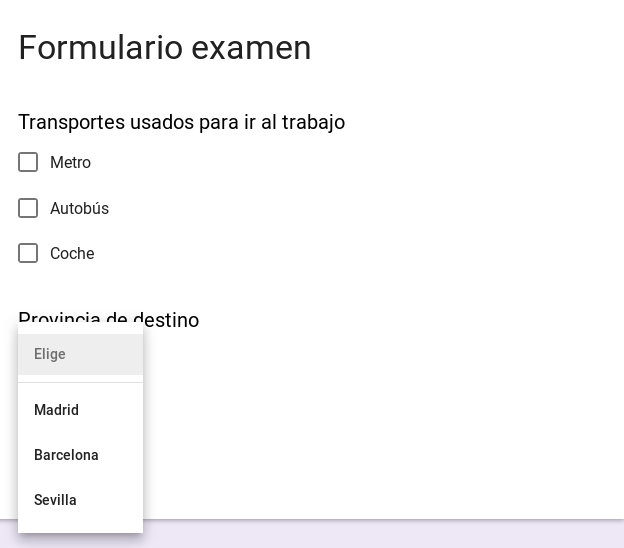
\includegraphics[scale=0.5]{examen-img/formulario.png}
\end{figure}

\break
\pregunta{Un conocido restaurante de la localidad ha encargado a nuestra empresa la realizaci�n de un portal de informaci�n donde puedan publicitar sus productos y servicios. Dado un Joomla ya instalado se solicita cumplir con las siguientes �rdenes de trabajo y documentar los pasos siguientes mediante las capturas de pantalla y explicaciones pertinentes.}{2.5}
\begin{enumerate}
\item{Modificar el estilo del front-end para que use ``Beez3'' (ya est� instalado).}
\item{Insertar un m�dulo para un nuevo men� en el que aparezcan dos enlaces: un enlace a los men�s del d�a, y otro enlace a la carta del restaurante.}
\begin{enumerate}

\item{    Crear el men�.}
\item{    Crear la categor�a Men� del d�a.}
\item{    Crear los �tems de men� necesarios.}
\item{    Crear el m�dulo y hacerlo visible.}

\end{enumerate}

\end{enumerate}
\end{document}
